\section{Implementation}\label{sec:web_ping_impl}

To collect data, we used the JavaScript image tag to load the images from the top 50 websites. To do the timing, the browser records the current time, loads the resources then marks the time when its done. Once all 50 resources have been loaded, the client packages the data into a \json and sends it via a web socket to the server. The server then stores the data in the database.

\begin{figure}
    \centering
    \small
    \begin{minted}{JavaScript}
function ping(url) {
  return new Promise(function (resolve, reject) {
    const start = (new Date()).getTime();
    const response = function () {
      let delta = ((new Date()).getTime() - start);
      resolve(delta);
    };
    request_image(url).then(response).catch(reason => reject(reason));
  });
}
    \end{minted}
    \caption{"Site ping" javascript ping function}
    \label{fig:web_ping_code}
\end{figure}

\subsection{Front end}

For the front end of the site, we chose to use the JavaScript Library D3.js to draw all of the maps. D3 is a data driven library specifically designed for data visualization of large \json data-sets. To draw the basic map, D3 loads in a \json file of the map and then draws and colors it. To draw the points for the city map, like the one below, the data gets passed into D3 in the form of \texttt{\small [\{favicon: "facebook.com", avg\_rtt: 1.1, city: "Boston", latitude: 0.0, longitude: 0.0\}]}. D3 then converts the longitude and latitude to coordinates on the screen and uses a a color gradient based on the \rtt to determine the color of the dot. Initially, we use the absolute minimum and maximum values of the data to determine the limits of the gradient, but we found that color gradients would often get skewed towards the outliers. To solve this problem, we switched to using the minimum and maximum of the inter-quartile range of the data set for the color gradient. All of the points in the lower and upper whiskers are displayed as pure red or pure white. This makes the graph not nearly as effected by outliers while still being fast enough that it can be done live, as opposed to z-score filtering for example.
% In the middle: Web sockets for data

\begin{figure}
    \centering
    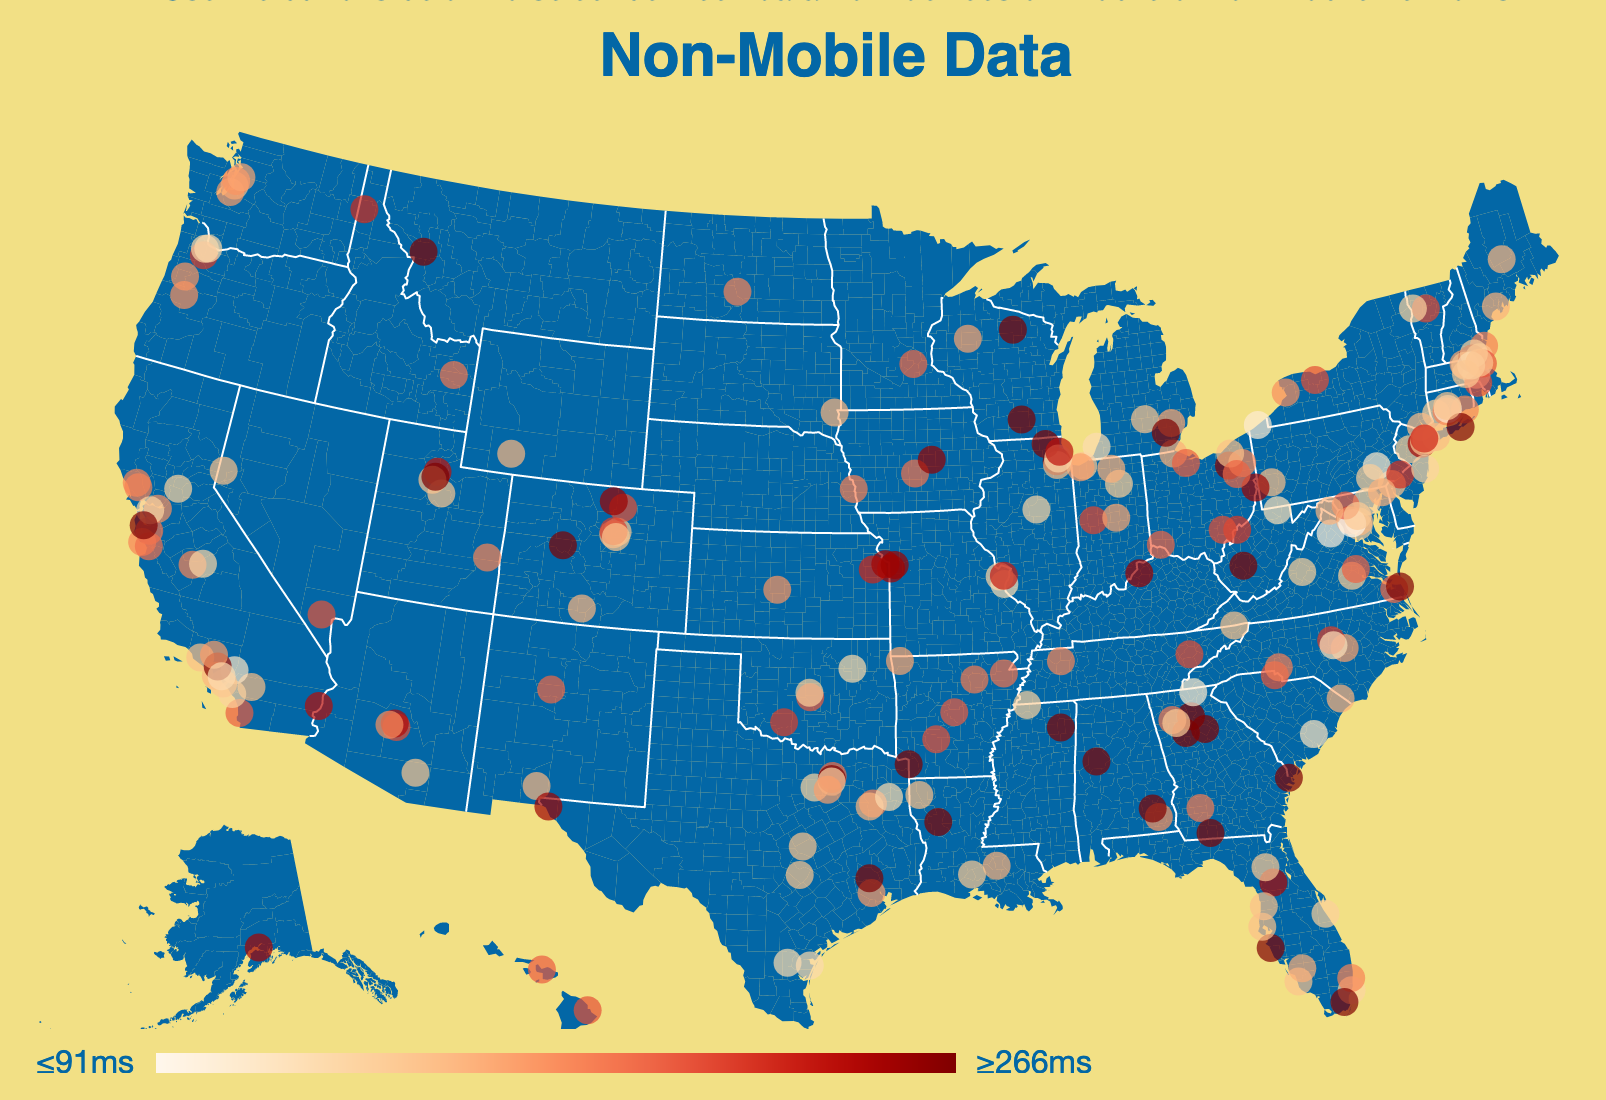
\includegraphics[width=\textwidth]{siteping/cityview.png}
    \caption{The city view from the website}
    \label{fig:siteping_city}
\end{figure}

\subsection{Back end and Database}

When a client sends data back to the server, the server will use the MaxMind \ip geolocation database to retrieve the users latitude and longitude. All of this information is then stored in the database and is also sent via web sockets to all of the other clients connected so that there map will be updated in real time. For the back-end database, we chose to use MongoDB to host all of our data and then query it when a new client connects. We chose MongoDB because of its simple and free cloud hosting platform known as Atlas, as well as the ease of integration with NodeJS. The backend web server is a NodeJS server hosted on an \ecc instance.

\subsection{Distribution}

We tried multiple different ways to get the site out to people all across the United States. To track engagement and distribution on the site, we used googles free analytics tools known as "Google Analytics." Google Analytics works because we embedded a block of JavaScript code that loads when the page loads. It then gathers information about the user's browser and other cookies that have been installed and uses that to determine where the user came from and how long they remain on the site. Finally, they encode the data into the metadata of a request for a one pixel image \cite{GoogleGoogleOverview}.

\subsubsection{Reddit}

The first technique we tried was to post the site on the popular Internet message board, Reddit. We posted in two communities, \href{https://reddit.com/r/dataisbeautiful}{/r/dataisbeautiful} which has around 14.2 million followers and \href{https://reddit.com/r/samplesize}{/r/samplesize} which has 121k followers. Unfortunately, posting on Reddit proved unsuccessful proved to be somewhat unsuccessful and gained us around 10 views. The primary reason why this occurred is that many people sort by popular posts, and our post did not get many upvotes, and therefore did not appear in very many peoples' view. 

\subsubsection{Facebook}

One of our most successful methods for deploying the site was through Facebook. Initially, one of our members posted it on his own personal page and we received a few views. Following soon after that, a family member posted the link into the WPI parents Facebook group which resulted in 125 views, all across the \us. Finally, a group member posted the link to four of the WPI undergraduate class Facebook groups, and resulted in us getting about 70 hits to the site. We intentionally waited to post to the \wpi undergraduates Facebook group until winter break had started, so as to maximize the geographic diversity.

\begin{figure}[h]
    \centering
    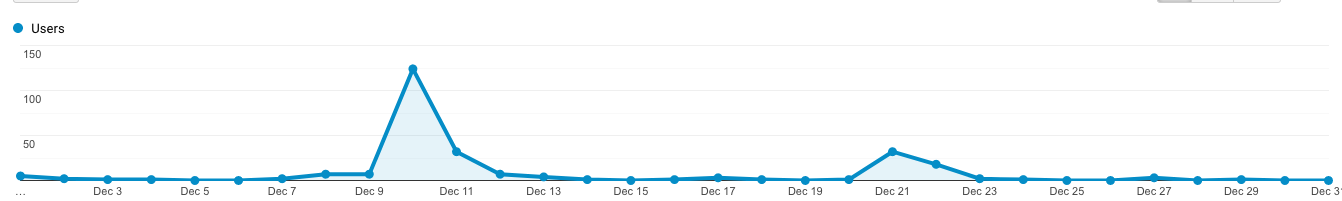
\includegraphics[width=\textwidth]{siteping/usage/facebook-usage.png}
    \caption{Facebook site visit}
    \label{fig:siteping_facebook_usage}
\end{figure}

\subsubsection{Amazon Mechanical Turk}

To reach people in states that we were lacking data for, we turned to paying people using Amazon's Mechanical Turk service. Mechanical Turk is a crowd sourcing platform that allows people to pay others to complete small online tasks. We used it to fill in gaps in our data by paying between 1 and 50 cents for users in states that we had no or very little data for. When someone chose to pick up our task, they would be directed to a special URL on the site ping website. When they clicked "collect data" and then waited for a set amount of time for data to be collected they would receive a token which they would copy and paste into Mechanical Turk to ensure that they actually completed the task. The actual tokens are generated using the JavaScript web token module for NodeJS. With Mechanical Turk we received 221 visits from Mechanical Turk and they helped fill in 47 of the 50 states.

\begin{figure}[h]
    \centering
    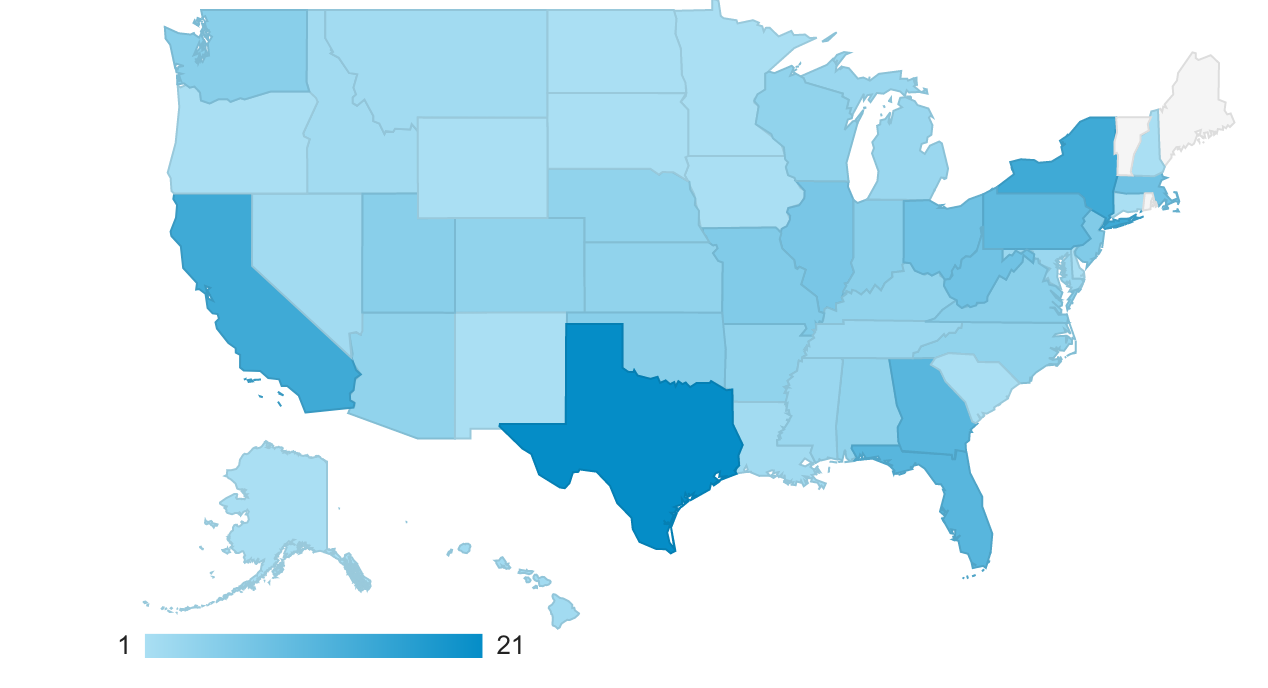
\includegraphics[width=\textwidth]{siteping/usage/mturk-distribution.png}
    \caption{Involvement from Mechanical Turk by state}
    \label{fig:siteping_mturk_distribution}
\end{figure}

\subsubsection{Email}
